\section{Conceptual design options} \label{ch:options}
This chapter will discuss the five design concepts that will be considered in this report. First the selection of concepts based on the shape, mission duration and controls system design option trees is made. In section \ref{sec:conf} the five selected configurations are sketched and described. A simple load analysis is given in the form of \gls{fbd} to gain insight in the functioning of each of the concepts. The following five design are consequently used for analysis in the relevant chapters of this report. Finally the control systems corresponding to the each of the shape configurations are discussed in chapter \ref{sec:ccs}.

\subsection{Concept selection}
 From the \acrfull{br} three \glspl{dot} were obtained for the design of the \gls{hiad}. In these designs concepts; shape, mission duration and control system are considered. This yielded a set of all the individual design options. These options are shown in Fig. \ref{fig:dotshape} to \ref{fig:dotcontrol}. From these \glspl{dot} a feasible set of design options can be obtained. In Fig. \ref{fig:dotshape} six deemed feasible concept configurations can be seen. This can consequently be combined with three possible control systems from Fig. \ref{fig:dotcontrol}. The mission duration varies for all concepts and is therefore considered separately for every design concept. 

\begin{figure}[H]
%\centering
\hspace{-23mm}
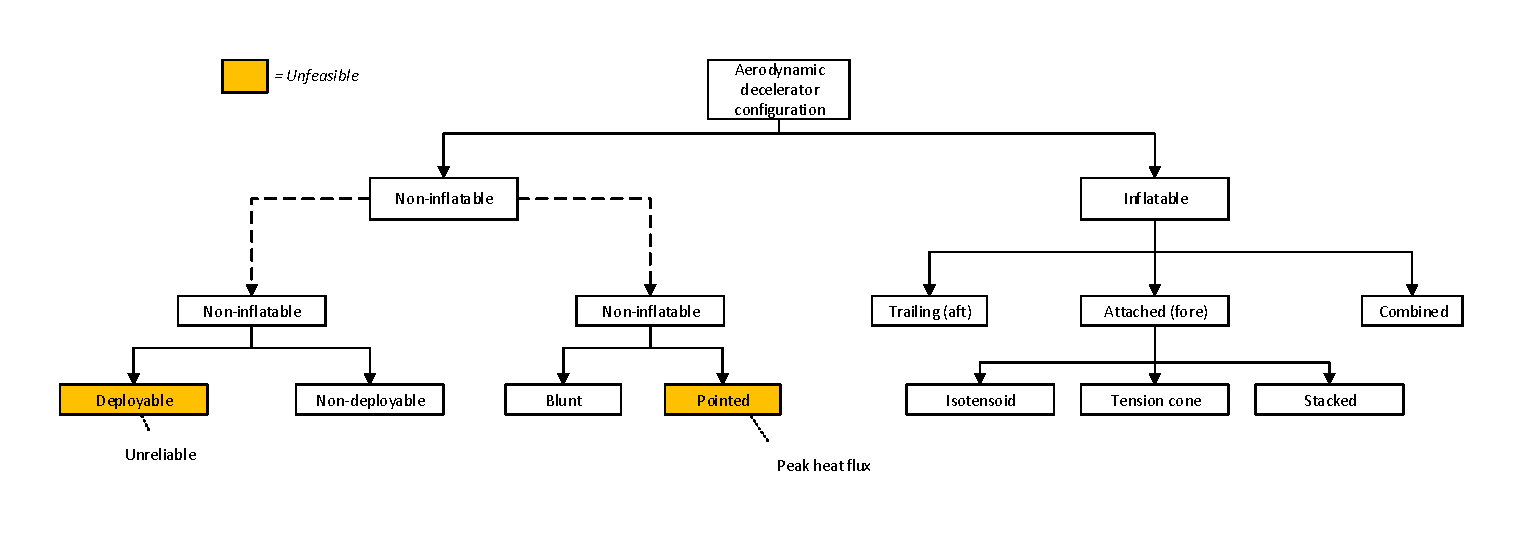
\includegraphics[width = 1.25\textwidth]{Figure/DOT_configuration.pdf}
\vspace{-5mm}
\caption{\acrlong{dot} for entry vehicle configurations}
\label{fig:dotshape}
\end{figure}

\begin{figure}[H]
\centering
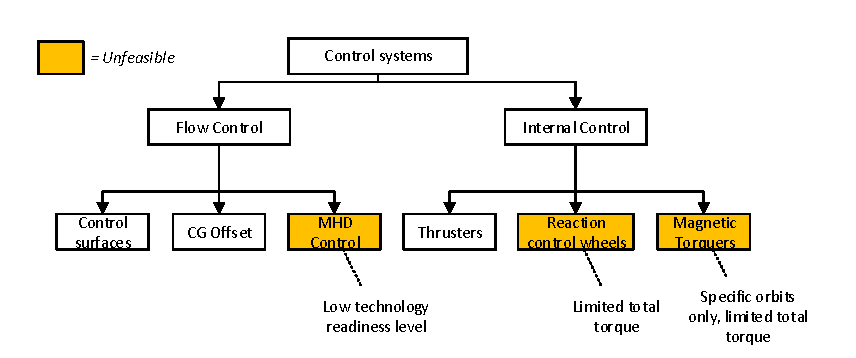
\includegraphics[width = 0.93\textwidth]{Figure/DOT_control.pdf}
\vspace{-5mm}
\caption{\acrlong{dot} for control systems}
\label{fig:dotcontrol}
\end{figure}

\begin{figure}[H]
\centering
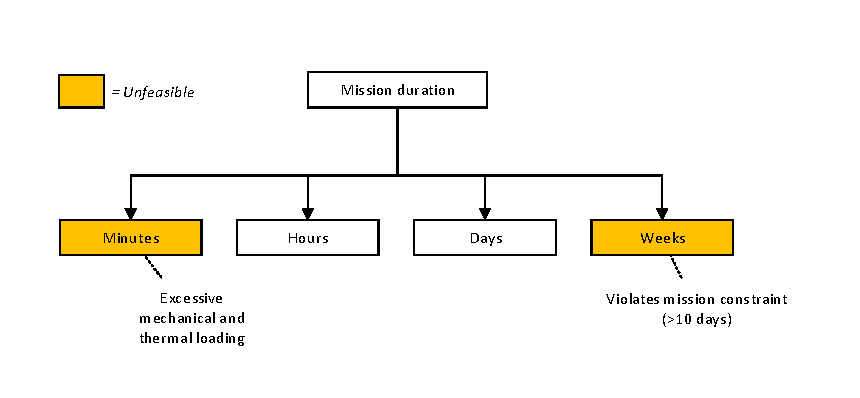
\includegraphics[width = 1.0\textwidth]{Figure/DOT_missionduration.pdf}
\vspace{-5mm}
\caption{\acrlong{dot} for mission duration}
\label{fig:dotduration}
\end{figure}

From the eighteen options yielded by combining the feasible shapes and control systems shown in Figures \ref{fig:dotshape} and \ref{fig:dotcontrol} some may be disregarded immediately since they cannot practically be combined. For obvious reasons it is crucial that each concept configuration features at least one deemed feasible control system. From this point onward the concept shape will be considered leading. 

The control systems from Fig. \ref{fig:dotcontrol} are considered separately for each of these shapes. Due to infeasibility of exotic control concepts such as the, for now, deemed infeasible \gls{mhd} the control system can be integrated with each structure as the control systems themselves do not require strict geometric properties as would be required by for example \gls{mhd} control.

Table \ref{tab:designconcepts} shows the design options that will be considered within this report. The check-marked control systems are further investigated for their feasibility and performance within section \ref{sec:ccs}. It must be noted that the control configurations of Table \ref{tab:designconcepts} feature the primary control mechanism. These may always be appended later on in the design process, after the trade-off, if additional control systems increase the overall systems performance. 

\begin{table}[H]
	\caption{Generation of design concepts}
	\label{tab:designconcepts}
	\centering
		\begin{tabular}{|p{0.3\textwidth}|p{0.14\textwidth}|p{0.14\textwidth}|p{0.14\textwidth}|} \hline 
			\textbf{Concept} & \textbf{Thrusters}	& \textbf{\gls{cg} offset} &  \textbf{Control surfaces} \\ \hline \hline
			Stacked toroid   & \cmark	& \cmark &  \cmark \\ \hline
			Isotensoid		 & \cmark	& \cmark &  \xmark\\  \hline
			Tension cone	 & \cmark	& \cmark &  \cmark \\ \hline
			Trailing 		 & \xmark	& \xmark &  \cmark \\ \hline
			Combined 		 & \xmark	& \xmark &  \cmark \\ \hline
			Rigid  		   	 & \cmark	& \cmark &  \cmark \\ \hline
		\end{tabular}
\end{table}

From Table \ref{tab:designconcepts} it can be noted that all shape configurations are deemed feasible for at least one control system. To yield a total of five concepts the combined concept is disregarded.
 It is considered to be too similar to a Trailing concept. A trailing concept will still require a heat shield in front of the payload and can therefore be considered, is some aspects, a combined configuration as well. It is therefore considered that a deployable inflatable at the front will have no additional advantage. A small deployable will have a similar performance as the trailing configuration, but features the additional complexity of the front inflation system. A large frontal inflatable will however place the aft inflatable in the wake making it effectively useless. Removing the aft declarator will however yield a "simple" stacked toroid, Isotensoid or tension cone configuration. For these reasons the trailing concept will not be considered. 
 
 The infeasible combinations of control systems are further detailed in \ref{sec:ccs}, together with a general description of each set of control system. 

\subsection{Concept configurations} \label{sec:conf}
In this section a the global configuration of each of the final five shapes is considered. They are sketched and described shortly in the sections below. Moreover a simple \gls{fbd} is provided to gain insight in, where applicable, the structural principle of each of the concepts.

\textbf{Stacked toroid}

Fig. \ref{fig:conc_stacked} and \ref{fig:fbd_stacked} show the stacked toroid concept. A stacked toroid configuration features multiple inflatables which are stacked together to form the aeroshell. These inflatables are consequently covered with a thermal protection layer. In this design the payload is placed aft of the aeroshell.\

\begin{figure}[H]
\centering
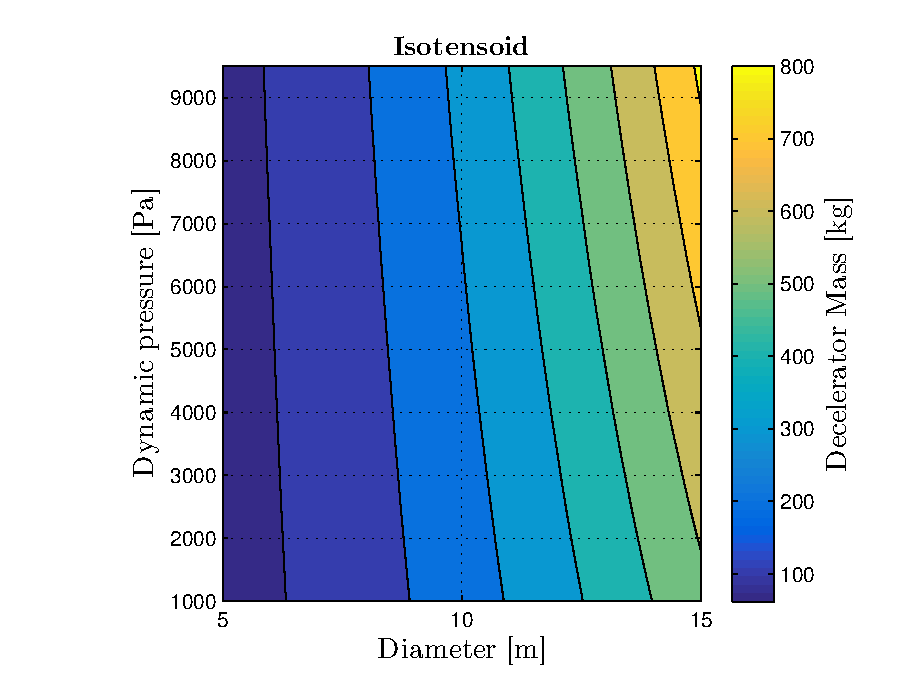
\includegraphics[width = 0.5\textwidth]{Figure/ISO_comp.eps}
\caption{A schematic view of a stacked toroid configuration}
\label{fig:conc_stacked}
\end{figure}

\begin{figure}[H]
\centering
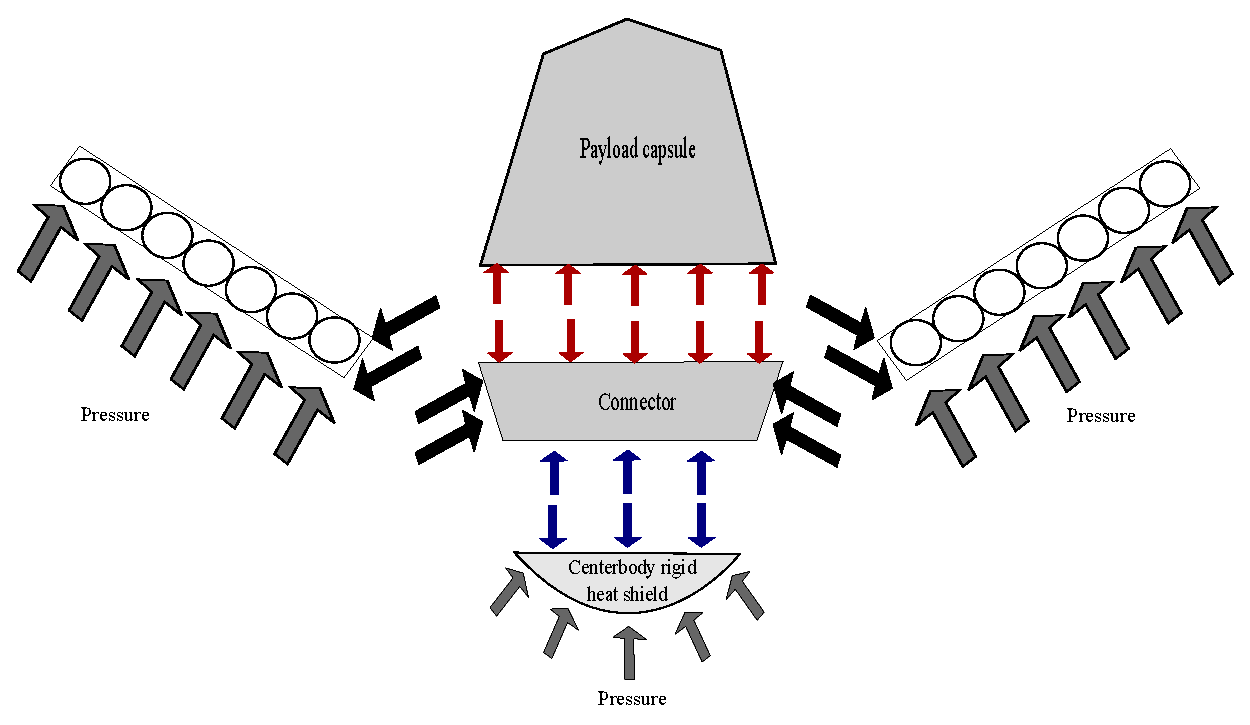
\includegraphics[width = 0.62\textwidth]{Figure/FBD_stacked.eps}
\caption{A \gls{fbd} of the stacked toroid configuration}
\label{fig:fbd_stacked}
\end{figure}


\textbf{Isotensoid}

An isotensoid configuration as displayed in Fig. \ref{fig:conc_iso} and \ref{fig:fbd_iso} features a single inflatable. This inflatable covers the whole of the payload. This inflatable is relatively large and is typically inflated using ram-air \cite{Smith2011}. 

\begin{figure}[H]
\centering
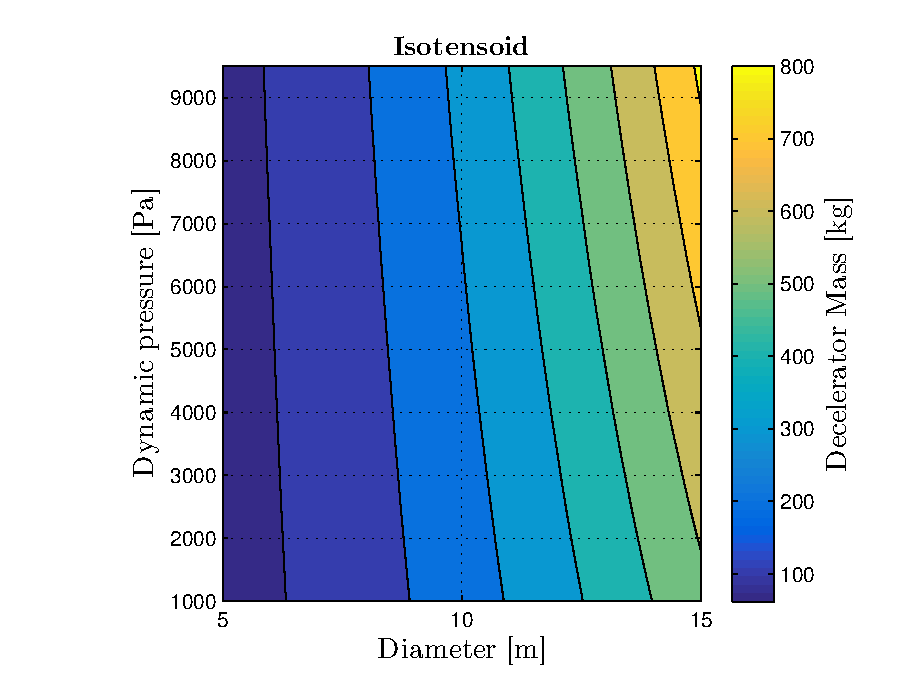
\includegraphics[width = 0.5\textwidth]{Figure/ISO_comp.eps}
\caption{A schematic view of a isotensoid configuration}
\label{fig:conc_iso}
\end{figure}

\begin{figure}[H]
\centering
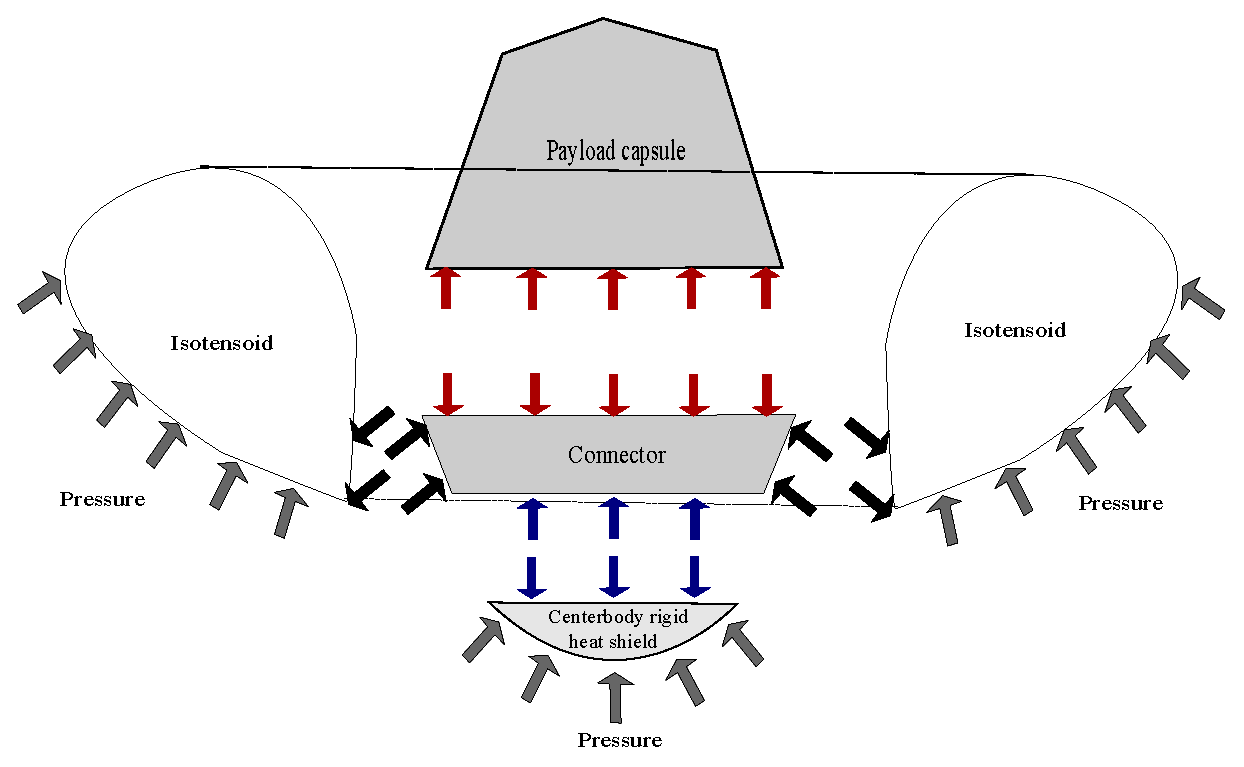
\includegraphics[width = 0.55\textwidth]{Figure/FBD_isotensoid.eps}
\caption{A \gls{fbd} of the isotensoid configuration}
\label{fig:fbd_iso}
\end{figure}

\textbf{Tension cone}

A tension cone, as shown in Fig. \ref{fig:conc_tension} and \ref{fig:fbd_tension}  again consists only of a single inflatable. In this case the inflatable is ring formed, using the ring to provide stiffness to a web spanned within. In this configuration the aeroshell is placed front of the payload, warping around it in some extend.

\begin{figure}[H]
\centering
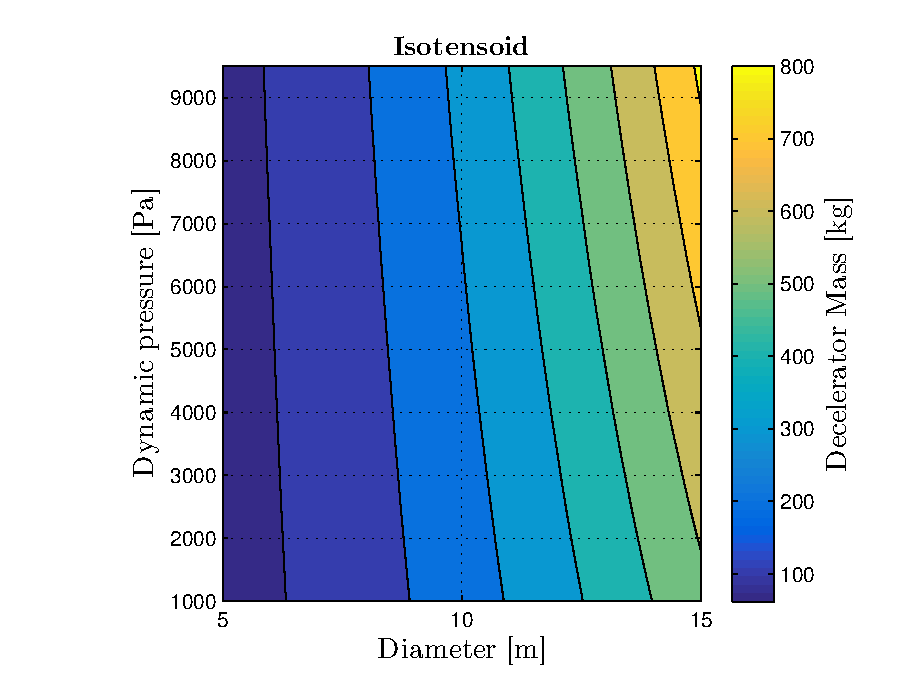
\includegraphics[width = 0.5\textwidth]{Figure/ISO_comp.eps}
\caption{A schematic view of a tension cone configuration}
\label{fig:conc_tension}
\end{figure}

\begin{figure}[H]
\centering
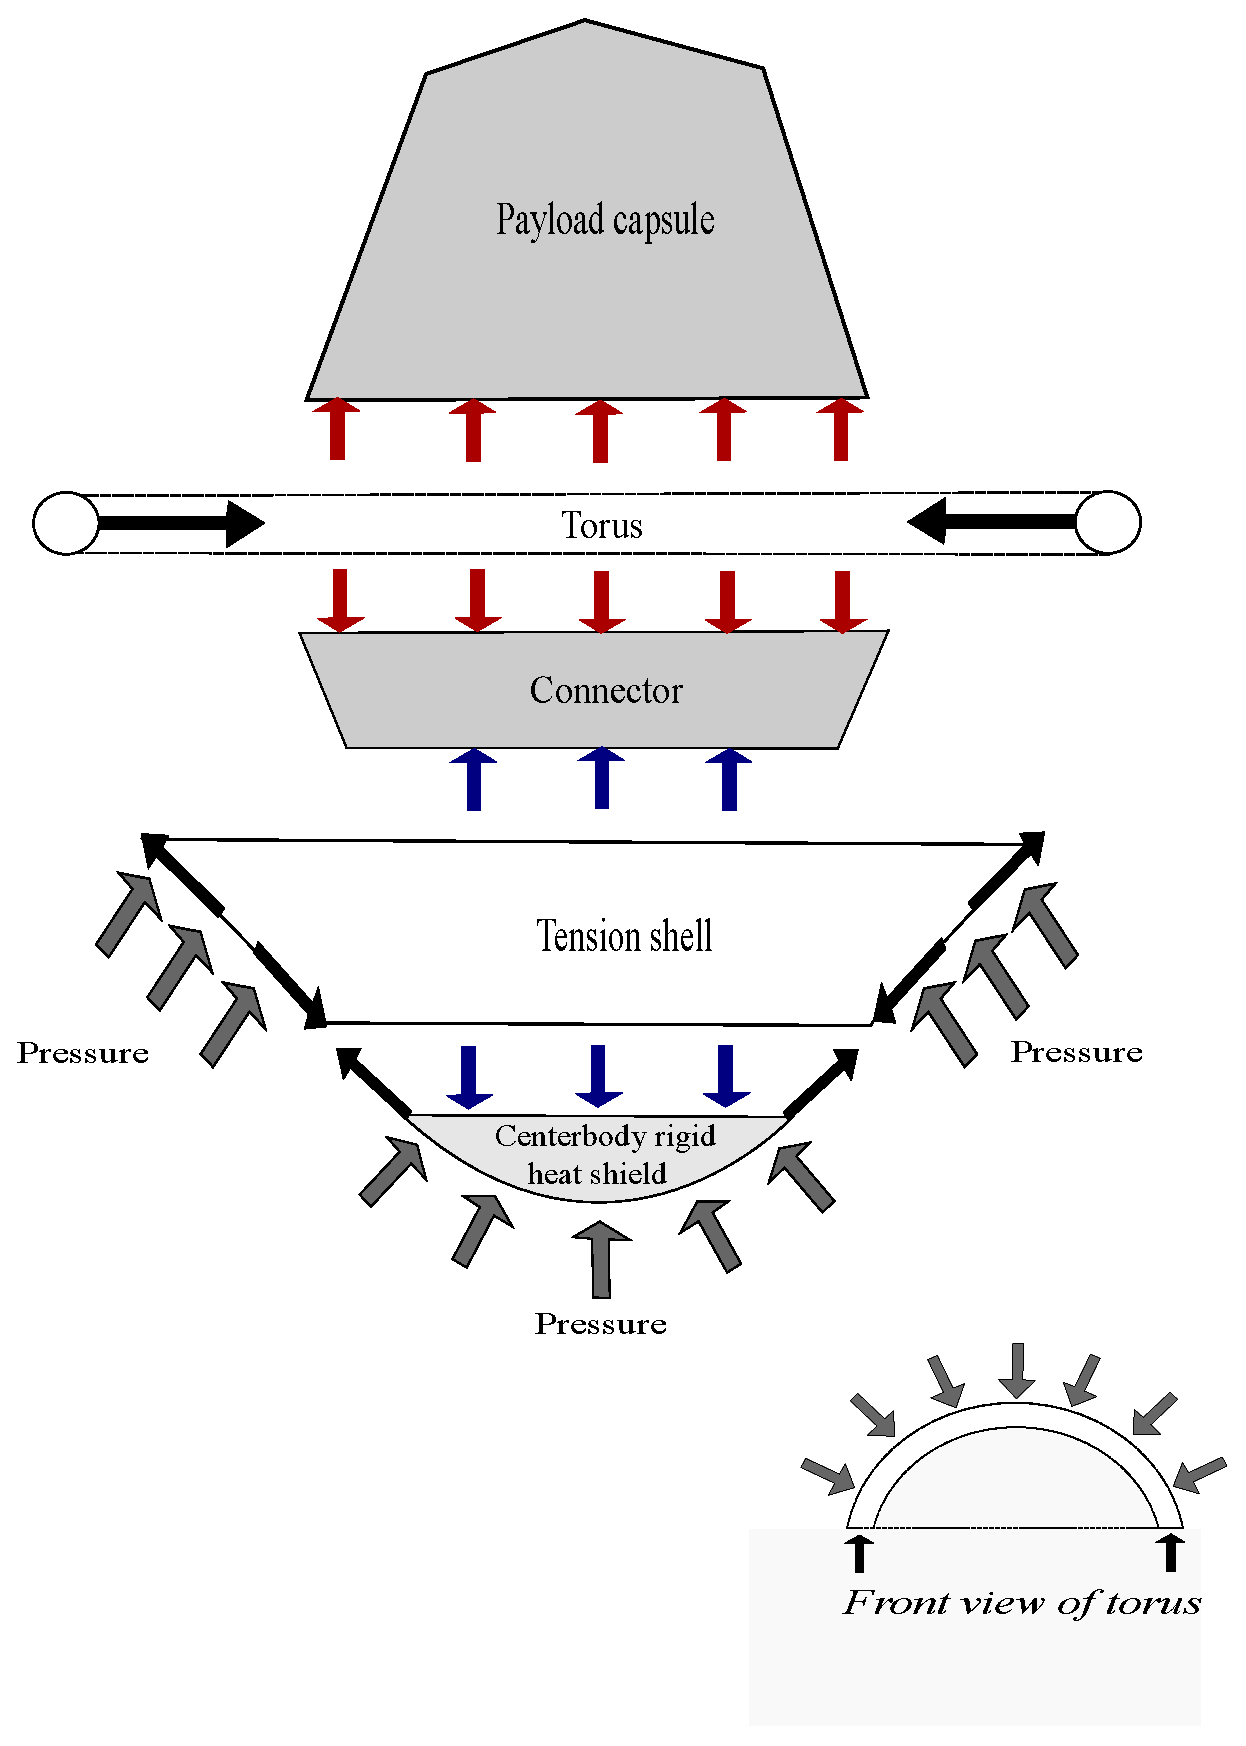
\includegraphics[width = 0.4\textwidth]{Figure/FBD_tensioncone.eps}
\caption{A \gls{fbd} of the tension cone configuration}
\label{fig:fbd_tension}
\end{figure}

\textbf{Trailing}

Fig. \ref{fig:conc_trailing} \ref{fig:fbd_trailing} show a trailing configuration. A Trailing configuration consist of two parts. A aft placed inflatable, typically referred to as the the trailing, and a front placed rigid heatshield. Since the inflatable is aft placed the payload is directly exposed to the atmosphere requiring the addition of the rigid heatshield. The shock waves induced by the front of the payload consequently create a wake aft of the payload. A typical trailing device is therefore ring formed to stay out of this wake is also displayed by Fig. \ref{fig:conc_trailing}. This is also the trailing configuration as treated within this report.

\begin{figure}[H]
\centering
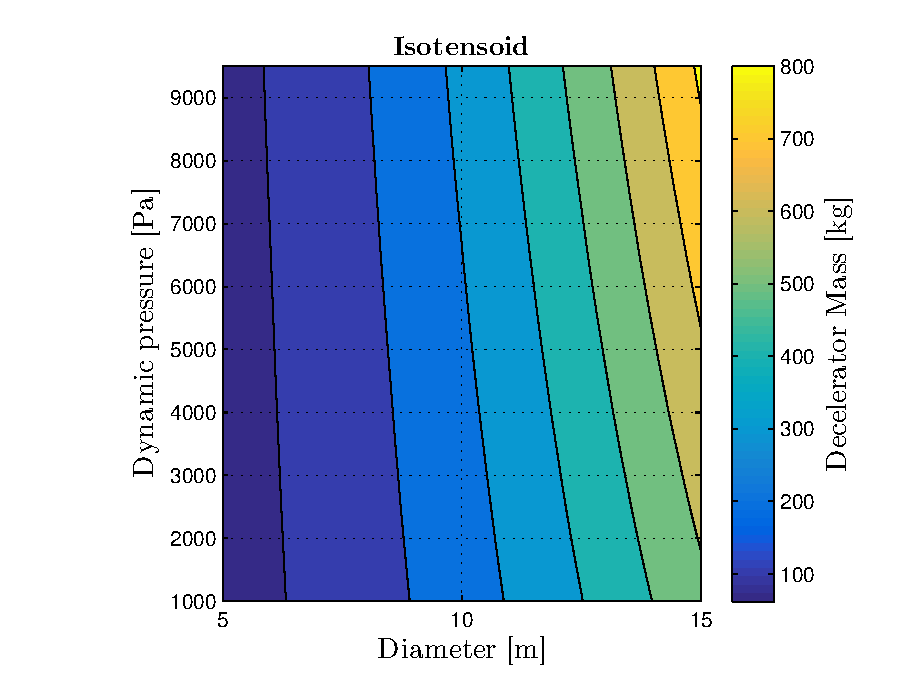
\includegraphics[width = 0.5\textwidth]{Figure/ISO_comp.eps}
\caption{A schematic view of a trailing configuration}
\label{fig:conc_trailing}
\end{figure}

\begin{figure}[H]
\centering
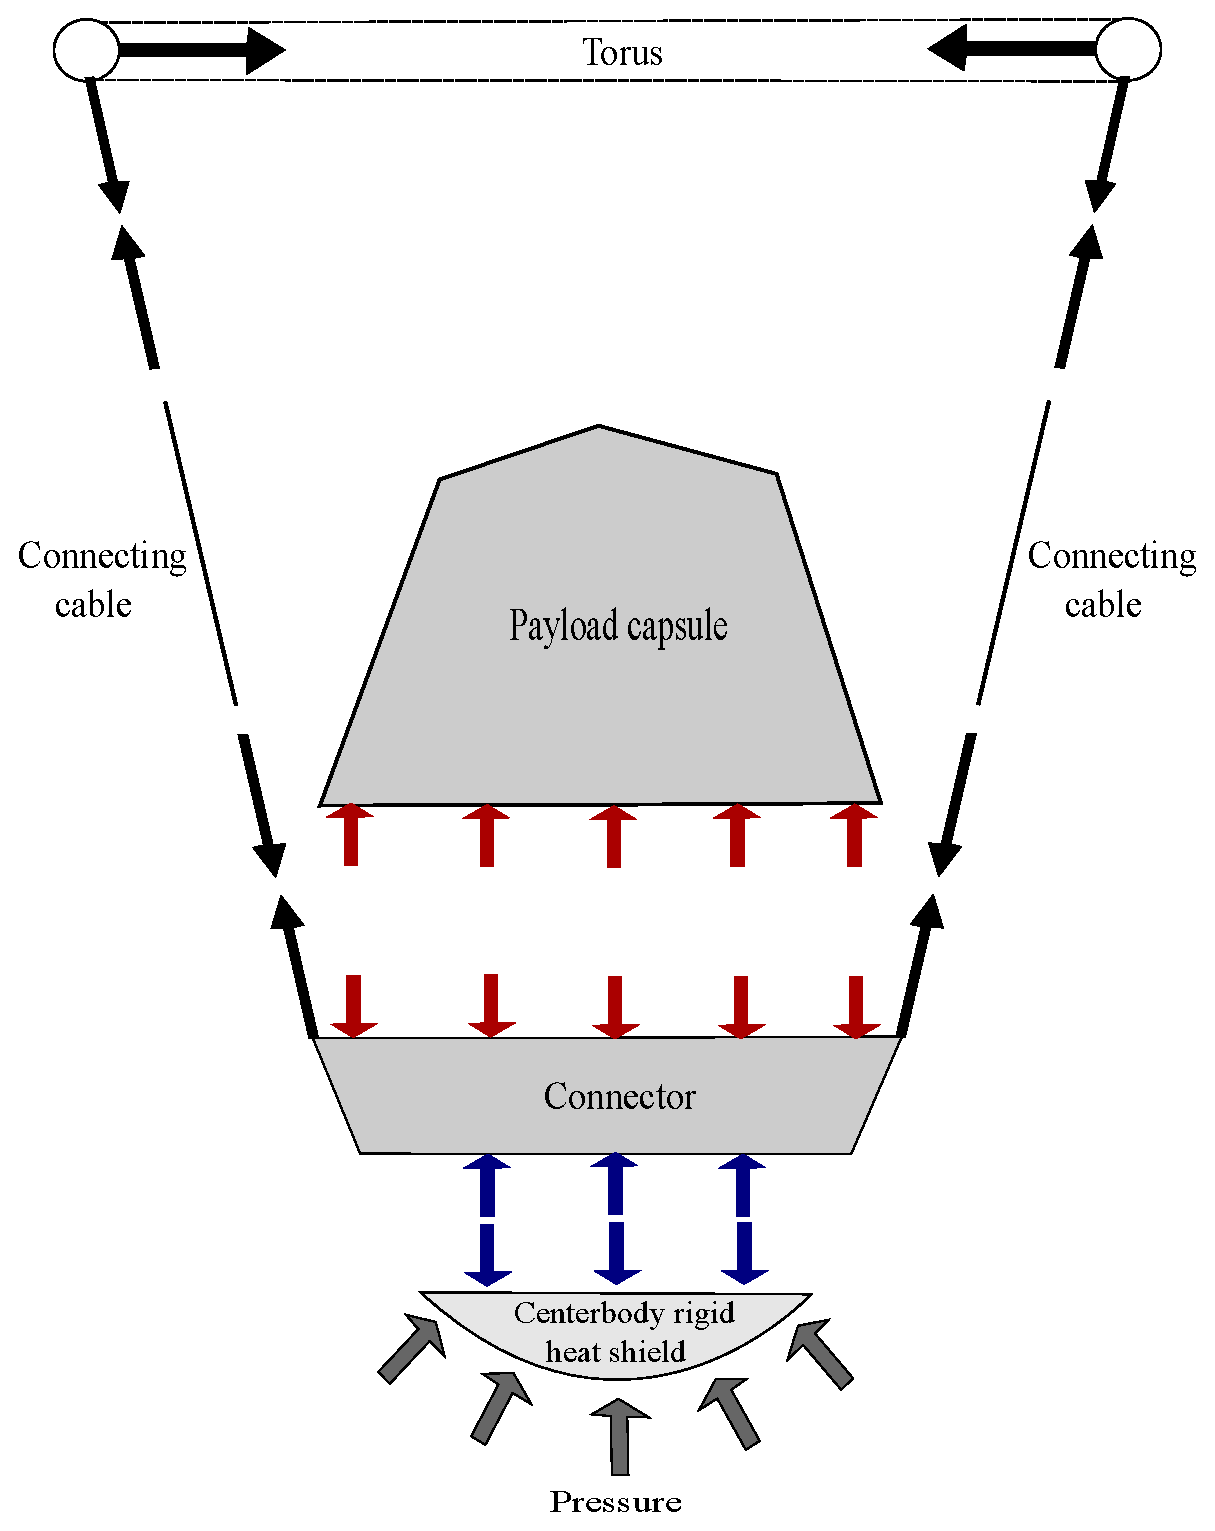
\includegraphics[width = 0.4\textwidth]{Figure/FBD_trailing.eps}
\caption{A \gls{fbd} of the trailing configuration}
\label{fig:fbd_trailing}
\end{figure}

\textbf{Rigid}

The rigid configuration is the most typical configuration and frequently used by returns to the earth atmosphere such as in the Apollo, Soyuz or planned Orion mission. Fig. \ref{fig:conc_rigid} and \ref{fig:fbd_rigid} show the Rigid configuration. This design features a rigid heatshield in front of the payload and is the only concept featuring no inflatable parts.

\begin{figure}[H]
\centering
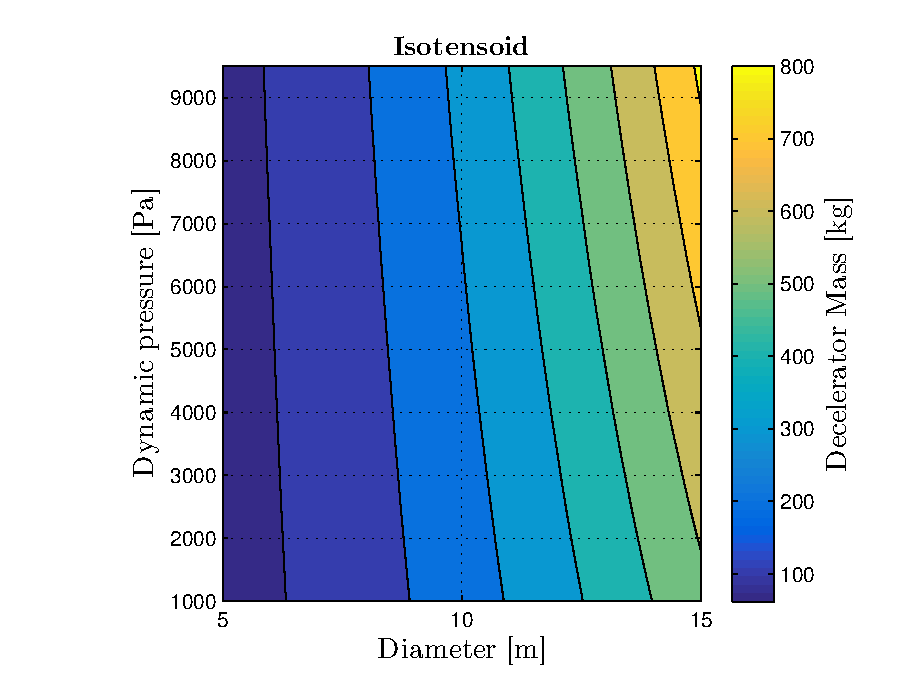
\includegraphics[width = 0.5\textwidth]{Figure/ISO_comp.eps}
\caption{A schematic view of a rigid configuration}
\label{fig:conc_rigid}
\end{figure}

\begin{figure}[H]
\centering
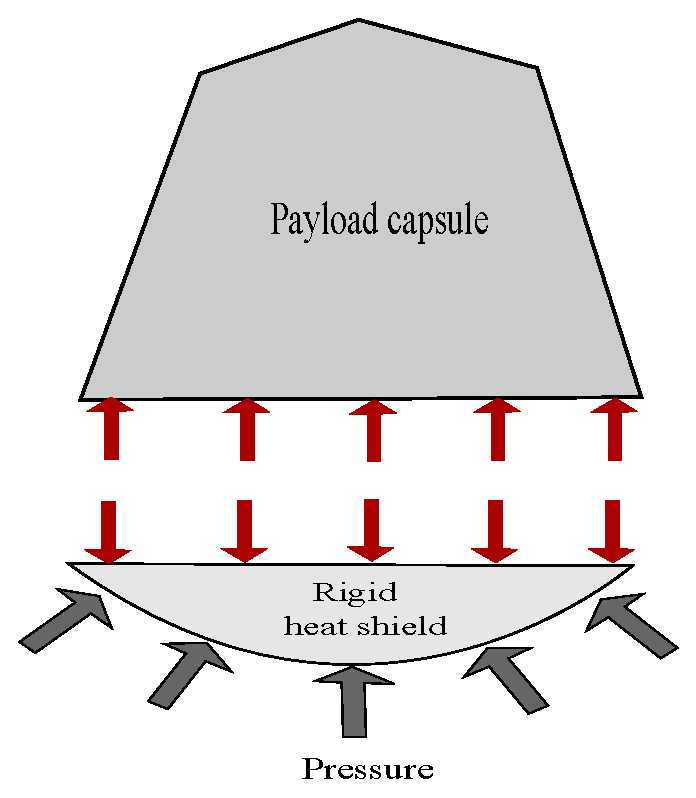
\includegraphics[width = 0.3\textwidth]{Figure/FBD_rigid.eps}
\caption{A \gls{fbd} of the rigid configuration}
\label{fig:fbd_rigid}
\end{figure}

\subsection{Concept control systems} \label{sec:ccs}
This section discusses the control systems for each of the control systems of the design option tree. This is related to the shapes of each of the concepts also explaining the checkmarks and crosses of Table \ref{tab:designconcepts}

\subsubsection{\gls{cg} offset}
A centre of gravity offset can be used in two ways. A static centre of gravity offset which is typically employed, and a actively employed \gls{cg} offset system. The latter is already demonstrated in the \gls{irve}-3 mission \cite{Dillman2012} , however considering smaller payload module mass fractions. Applying a \gls{cg} offset yields  a non symmetric body, creating a lift vector. In a \gls{cg}-offset control system this property is actively used for the control of the system. 

The use of a \gls{cg} does however have speed limitations as changes is centre of gravity are slow.

The usage of a active \gls{cg} offset systems for the trailing and combined configuration is not deemed feasible due to the existence of aft the elements which are connected with a non rigid combination.


For the trailing concept a \gls{cg} offset is a control system that is not deemed feasible
\subsubsection{Thrusters}
Thrusters are the only deemed feasible internal control system and is hence always featured on the spacecraft. For the part of the mission up to the first entry into the Martian atmosphere thruster will thus be used in any case. Thrusters can however also be employed as a primary control surface for which the mass and usage of the systems is obviously increased.  

Thruster are deployed in pairs for the control of the spacecraft such that they can deliver pure torque. The amount of torque is a linear function of the relative distance between the thrusters and is constrained for this design by launcher constraints. 

Thrusters are not considered for the trailing and combined configuration. Due to the aft elements of these designs thruster cannot be considered as the primary control mechanism. Due to the large moments of inertia (due to aft elements) and very high stability of the aft systems (e.g. compare to a parachute) thrusters cannot be considered due their inefficiency. 

\subsubsection{Control surfaces}
Control surfaces have been subdivided into two forms; body flaps and morphing of the whole structure which are both covered below.

\paragraph{Body flaps}
A control system with body flaps features deployable surfaces to control the flow around the spacecraft. Body flaps have previously been deployed at for example the Space Shuttle missions. It must however be noted that the usage was limited to lower Mach numbers at higher atmospheric densities. As such it is possible control concept for the rigid structure.

Body flaps on inflatable structures have not yet been featured and are not deemed feasible. Since body flaps need to based inside the flow positioning is not possible. In these designs the inflatable is the part placed within the flow. Do to the nature of deployment and the structural layout of these systems body flaps are not deemed feasible.

\paragraph{Morphing}
In morphing concepts the whole external shape is changed to control the spacecraft. This is not possible for rigid structures as no morphable parts exist, from the perspective of rigid decelerator structure. 
 For the inflatable structures morphing is deemed possible for with the exception of the isotensoid design and is already being investigated \cite{Hughes2011}. In the isotensoid design the whole outside is covered by inflatable. The whole inflatable can thus only e formed by usage of the gas inside. This is however not deemed possible due to the usage of ram-air as inflation mechanism.

Morphing of the trailing ballute configuration would be done via the payload-ballute connection much like for example a parachute.